\documentclass[a5paper]{article}
\usepackage[a5paper, top=8mm, bottom=8mm, left=8mm, right=8mm]{geometry}

\usepackage{polyglossia}
\setdefaultlanguage[babelshorthands=true]{russian}

\usepackage{fontspec}
\setmainfont{FreeSerif}
\newfontfamily{\russianfonttt}[Scale=0.7]{DejaVuSansMono}

\usepackage[font=scriptsize]{caption}

\usepackage{amsmath}
\usepackage{amssymb,amsfonts,textcomp}
\usepackage{color}
\usepackage{array}
\usepackage{hhline}
\usepackage{cite}

\usepackage[hang,multiple]{footmisc}
\renewcommand{\footnotelayout}{\raggedright}

\PassOptionsToPackage{hyphens}{url}\usepackage[xetex,linktocpage=true,plainpages=false,pdfpagelabels=false]{hyperref}
\hypersetup{colorlinks=true, linkcolor=blue, citecolor=blue, filecolor=blue, urlcolor=blue, pdftitle=1, pdfauthor=, pdfsubject=, pdfkeywords=}

\newlength\Colsep
\setlength\Colsep{10pt}

\usepackage{tabu}

\usepackage{graphicx}
\usepackage{indentfirst}
\usepackage{multirow}
\usepackage{subfig}
\usepackage{footnote}
\usepackage{minted}
\usepackage{xcolor}

\tabulinesep=1.2mm

\newcommand{\attribution}[1] {
\vspace{-5mm}\begin{flushright}\begin{scriptsize}\textcolor{gray}{\textcopyright\, #1}\end{scriptsize}\end{flushright}
}

\sloppy
\pagestyle{plain}

\title{Работа с сетью, высокий уровень}
\author{Юрий Литвинов\\\small{y.litvinov@spbu.ru}}

\date{12.10.2021}

\begin{document}

\maketitle
\thispagestyle{empty}

\section{Теоретическое введение}

Начнём с краткого теоретического введения в протоколы прикладного уровня, в частности, HTTP, поскольку именно на нём базируется работа с высокоуровневыми сетевыми ресурсами.

По доброй традиции этого курса, <<забудьте всё, что вам рассказывали в предыдущей лекции>> --- в современном мире если вы пользуетесь <<голыми>> сокетами под .NET, скорее всего, вы делаете что-то не так. TCP и UDP обеспечивают транспорт, они слишком низкоуровневые для прикладного использования. Вся полезная работа делается протоколами приколадного уровня, многие из которых широко распространены и имеют хорошую поддержку в библиотеках и даже в стандартных библиотеках языка. Например, вам не надо формировать правильный пакет, чтобы сделать DNS-запрос, скорее всего, вам не надо будет делать вручную DNS-запросы вообще. Помимо DNS, широкоиспользуемых протоколов ещё очень много:

\begin{itemize}
    \item Электронная почта: SMTP, IMAP, POP3. SMTP (Simple Mail Transfer Protocol) используется в основном для отправки сообщений почтовому серверу, IMAP (Internet Message Access Protocol) --- протокол управления почтовым ящиком, позволяющий, в частности, манипулировать почтой, не получая её целиком на клиента. POP3 (Post Office Protocol Version 3) --- протокол получения почты.
    \item Различные виды удалённого вызова: WCF, Apache Thrift, gRPC и т.д. --- протоколы и реализующие их библиотеки, которые позволяют вызывать методы объектов на удалённой машине так, будто они находятся в вашем адресном пространстве. Как правило, достаточно продвинуты, чтобы даже автоматически генерировать код, который потом можно будет вызывать, по описанию сервиса (которое в случае с WCF даже можно получить автоматически). Берут на себя все вопросы, связанные с авторизацией и шифрованием.
    \item WWW: HTTP, HTTPS --- протоколы передачи веб-страниц и подобных данных. Также используются как транспортные для других прикладных протоколов.
    \item Стриминг: RTP (Real-time Transport Protocol), RTCP (RTP Control Protocol) --- протоколы стриминга аудио и видео, используются совместно. RTP собственно доставляет контент, RTCP управляет процессом и передаёт статистику. Работают поверх UDP.
    \item P2P (Peer-to-Peer, <<одноранговые сети>>) и доставка контента: BitTorrent --- протокол распределённой передачи файлов, когда один файл может качаться сразу с нескольких (как правило, нескольких десятков) разных источников, тем самым позволяя получать очень неплохие скорости доставки файлов даже в ситуациях, когда нет выделенных серверов с широким каналом, способных эти файлы быстро отдавать. Чрезвычайно технически интересный и полезный протокол, но ассоциируется с пиратством.
\end{itemize}

\subsection{Как работает браузер}

Рассмотрим подробнее протокол HTTP, на примере его использования в браузере. Вот что происходит <<под капотом>>, когда вы заходите на свой любимый вконтакт или куда-то ещё:

\begin{enumerate}
    \item Определяет URL, указывающий на желаемую страницу. URL может быть вручную введён в адресную строку, получен из ссылки, из истории просмотра или ещё откуда-то.
    \item Выполняет DNS-запрос на доменное имя из URL, узнаёт IP. Про это было подробно в предыдущей лекции, напомним лишь, что DNS-запрос может потребоваться не один.
    \item Устанавливает TCP-соединение с портом 80 целевой машины.
    \item Отправляет HTTP-запрос на получение файла. Про то, как выглядят HTTP-запросы буквально чуть-чуть позже, сейчас достаточно сказать, что HTTP --- текстовый протокол, причём довольно простой (так что в telnet просимулировать HTTP-пакет ничего не стоит, иное дело, что подавляющее большинство серверов принимают только HTTPS-соединения, а HTTPS шифрованный).
    \item Получает ответ от сервера с HTML-страницей --- в виде ответного пакета HTTP. Страница --- это просто текст (на самом деле даже поток байт) в теле пакета.
    \item Если страница содержит URL, необходимые для её отображения (например, ссылается на картинки, скрипты, стили и т.д.), браузер повторяет процесс для каждого требуемого URLа. Протокол HTTP/2 умеет умнее, заранее отправляя ресурсы, которые могут понадобиться при рендеринге страницы, но HTTP 1.1, который до сих пор очень активно используется, так не умеет.
    \item Браузер отображает (рендерит) страницу, отдаёт скрипты на интерпретацию во встроенный интерпретатор JavaScript, при необходимости запускает плагины.
    \item Если новых запросов некоторое время не поступает, браузер разрывает соединение с сервером.
\end{enumerate}

\subsection{Протокол HTTP}

HTTP (Hypertext Transfer Protocol) --- простой текстовый протокол поверх TCP, изначально предназначавшийся для передечи веб-страниц. Работает по схеме <<запрос-ответ>>: клиент открывает TCP-соединение, отправляет по нему запрос в виде HTTP-пакета, получает ответ от сервера и на этом коммуникация заканчивается (хотя и может быть повторена в рамках того же соединения). Формат запроса такой:

\begin{minted}{text}
    <Метод> параметр <версия протокола>
    <Заголовки>
    <Тело запроса>
    <Пустая строка>
\end{minted}

Метод --- один из восьми стандартных методов (GET, HEAD, PUT, POST, DELETE, TRACE, CONNECT, OPTIONS), говорящий, что клиент хочет от сервера. Параметр --- это обычно URL. Версия протокола --- жумаю, понятно.

Заголовки --- это набор строковых пар <<ключ-значение>>, по одной паре на строку. Нужны для передачи дополнительной информации для обработки запроса. Например, кто мы или в какой кодировке мы хотим ответ.

Тело запроса --- собственно, данные, отправляемые на сервер, могут быть чем угодно, но как правило, используется . Может быть пустым.

Пустая строка служит признаком конца передачи одного запроса.

Вот пример (слегка сокращённый) HTTP-запроса:

\begin{minted}{text}
    GET http://se.math.spbu.ru/SE HTTP/1.1
    Host: se.math.spbu.ru
    Connection: keep-alive
    Upgrade-Insecure-Requests: 1
    User-Agent: Chrome/68.0.3440.106 
    Accept: text/html,application/xhtml+xml
    Referer: http://se.math.spbu.ru/
    Accept-Encoding: gzip, deflate
    Accept-Language: ru-RU,ru;q=0.9,en-US;q=0.8,en;q=0.7
    
\end{minted}

А вот очень сокращённый ответ на такой запрос:

\begin{minted}{text}
    HTTP/1.1 200 OK
    Server: Zope/(Zope 2.10.6-final, python 2.4.6, linux2) ZServer/1.1 Plone/3.1.3
    Date: Sat, 01 Sep 2018 12:57:32 GMT
    Content-Length: 29068
    Content-Language: ru
    Expires: Sat, 1 Jan 2000 00:00:00 GMT
    Content-Type: text/html;charset=utf-8
    
    <!DOCTYPE html ...>
    <html xmlns="http://www.w3.org/1999/xhtml" xml:lang="ru"
          lang="ru">
      <head>
      </head>
      <body>
      </body>
    </html>
\end{minted}

Сервер нам ответил кодом 200 (что означает, что всё хорошо), сообщил, что он Zope такой-то версии, обозначил дату и время отправки ответа (это нужно для кеширования), но сказал, что содержимое страницы потеряет актуальность 1 января 2000 года (дата в прошлом, чтобы браузер не кешировал страницу). Также были присланы длина ответа и язык, кодировка и MIME-тип ответа (text/html). Дальше после пустой строки, отделяющие заголовки от тела, --- сама HTML-страница.

Какие методы в HTTP бывают и что делают (кстати, методы --- такие же и в HTTPS и в любых версиях протокола):

\begin{itemize}
    \item \textbf{GET} --- получить страницу либо вообще получить информацию о запрошенном ресурсе. Как правило, отправляется без тела, хотя стандарт тела не запрещает.
    \item \textbf{HEAD} --- получить только заголовок страницы. Якобы для того, чтобы браузер мог большой контент не качать, если всю страницу показывать пользователю не собирается, на практике не встречал.
    \item \textbf{PUT} --- залить новую страницу на сервер, либо вообще добавить ресурс куда-то. Обычно посылается с телом, содержащим в себе добавляемый элемент.
    \item \textbf{POST} --- добавить что-нибудь к странице. Используется в веб-формах для отправки результата её заполнения, а также вообще как основной вид запроса, который что-то отправляет на сервер.
    \item \textbf{DELETE} --- удалить страницу или вообще удалить какой-то ресурс.
    \item \textbf{TRACE} --- отправить запрос обратно, ничего с ним не делая. Наверное, бывает полезно для отладки, чтобы посмотреть, в каком виде ваш запрос попадает на сервер (после разных прокси, глючащих прослушивалок ЦРУ и т.п.), на практике ни разу не видел.
    \item \textbf{CONNECT} --- подключиться через прокси. Тоже ни разу не использовал.
    \item \textbf{OPTIONS} --- узнать, что можно использовать на сервере. Тоже ни разу не использовал.
\end{itemize}

А вот коды ответов сервера. Они разделены на пять категорий, в зависимости от результата исполнения. Некоторые из этих кодов любой нормальный программист должен знать наизусть, они в этой таблице в колонке <<примеры>>:

\begin{tabu} {| X[0.3 l p] | X[0.5 l p] | X[1 l p] |}
    \tabucline-
    Код  & Значение         & Примеры                                                       \\
    \tabucline-
    \everyrow{\tabucline-}
    1xx  & Информация       & 100 --- сервер согласен обрабатывать запросы                  \\
    2xx  & Успех            & 200 --- запрос успешно обработан, 204 --- ответ пустой        \\
    3xx  & Перенаправление  & 301 --- страница перемещена, 304 --- возьмите из своего кэша  \\
    4xx  & Ошибка клиента   & 404 --- страница не найдена, 403 --- нет прав                 \\
    5xx  & Ошибка сервера   & 500 --- сервер упал, 503 --- попробуйте позже                 \\
\end{tabu}

Тут код 304 выглядит странно, но нужен для реализации такой функциональности: браузер, не будучи уверенным в том, что страница актуальна, шлёт на сервер GET-запрос со временем получения своей кешированной версии страницы, и сервер отвечает либо новой версией страницы, либо кодом 304, чтобы браузеру не надо было качать то, что у него и так есть. Сообщение с кодом 301 содержит информацию о том, куда страница перемещена, и браузер в этом случае делает новый запрос на новый адрес.

403 (forbidden)--- ошибка авторизации. Значит, запрос не содержит заголовка, позволяющего его опознать как запрос от авторизованного пользователя (обычно это какой-то токен авторизации, то есть случайная строка, которую сервер помнит, что отправлял клиенту). Все заголовки, связанные с безопасностью (даже логин-пароль) передаются прямым текстом как заголовки HTTP-запроса, в надежде на шифрование, обеспечиваемое HTTPS. Поэтому если вы общаетесь с сервером по <<голому>> HTTP (не HTTPS), никогда не передавайте свой логин-пароль и другую важную информацию. Их может прочитать любой, кто видит ваш пакет, начиная от вашего провайдера, заканчивая случайным бомжом, взломавшим ваш WiFi (это не так сложно сделать, протокол WEP ломается в считанные минуты, WPA2, который обычно нынче используется, взломать сложнее, но можно при желании).

Код 500 (internal server error) означает необработанное исключение в приложении, которое на стороне сервера обрабатывает ваш запрос. Обычно виноват автор сервера, но часто на практике это означает неправильно сформированный запрос со стороны клиента (например, если вы пытаетесь прикинуться iPhone, синхронизирующимся с облачным хранилищем чтобы утянуть чужие бэкапы, вы можете довольно часто получать ошибку 500 из-за неаккуратной поддержки протокола). Код 503 означает просто, что сервер перегружен.

\section{HTTP в .NET}

За работу с протоколом HTTP в .NET отвечает класс HttpClient, умеющий выполнять HTTP-запросы разными методами, поддерживающий заголовки, тело и т.д. Вот минимальный пример его использования: 

\begin{minted}{csharp}
class Program
{
    private static async Task Main(string[] args)
    {
        var httpClient = new HttpClient();

        var response = await httpClient.GetAsync("http://hwproj.me/");
        if (response.IsSuccessStatusCode)
        {
            var content = await response.Content.ReadAsStringAsync();
            Console.WriteLine(content);
        }
    }
}
\end{minted}

Однако ранее обсуждалось, что сеть принципиально ненадёжна, а этот код наивно надеется, что первый же запрос завершится успешно. Более типично использовать повторные запросы, но если ошибка вызвана тем, что сервер перегружен или сеть перегружена, то постоянные повторы только усугубят положение. Поэтому часто применяется техника <<экспоненциального отката>>:

\begin{minted}{csharp}
static async Task<string> DownloadStringWithRetries(string uri)
{
    using (var client = new HttpClient()) {
        var delay = TimeSpan.FromSeconds(1);
        for (int i = 0; i != 3; ++i) {
            try {
                return await client.GetStringAsync(uri);
            } catch {
            }
            await Task.Delay(delay);
            delay *= 2;
        }

        // Попробуем последний раз, дав ошибке распространиться
        return await client.GetStringAsync(uri);
    }
}
\end{minted}

Тут мы пытаемся выполнить запрос, если всё хорошо, то возвращаем результат. Если нет, ловим исключение, никак на него не реагируем (это важное исключение из правила, что надо всегда что-то делать с исключениями), делаем задержку и время задержки увеличиваем вдвое. То есть ели и вторая попытка не прошла, ждём две секунды, затем четыре, затем восемь. Если совсем всё плохо, повторяем операцию вне try/catch, чтобы она всё-таки упала и исключение было поймано выше.

\section{Веб-сервисы}

Рассказ про протокол HTTP был вовсе не для того, чтобы вы сели писать свой браузер (при большом желании это возможно, но зачем, есть полно готовых и хороших с открытым исходным кодом). Прежде всего HTTP в .NET служит транспортным протоколом для общения по схеме <<приложение-приложение>>, и уметь им пользоваться надо для того, чтобы обращаться к веб-сервисам.

Веб-сервисы --- это что-то вроде страниц в интернете, предназначенных не для браузеров, а для других приложений. Например,

\begin{itemize}
    \item программный интерфейс для облачных сервисов типа GMail, Google Drive, ВКонтакте, Twitter и т.д., позволяющий писать свои клиенты или автоматизировать частые операции. Очень многие приложения используют Google Drive для хранения своих данных, существует куча приложений для получения данных из соцсетей, в частности для нужд исследований по BigData и NLP. Сами официальные клиенты этих сервисов как правило используют тот же программный интерфейс, что и доступный стороноим разработчикам, плюс-минус незадокументированные параметры и немного специальных вызовов, которых тоже нет в документации. Надо понимать, что протокол общения официального клиента и сервера может легко прочитать каждый, так что ничего прямо секретного там быть и не может.
    \item Публичные API для сторонних приложений. Например, есть веб-сервисы, сообщающие актуальные курсы валют или погоду. И не совсем публичные API для проприетарных сетевых приложений, например, для бэкапов смартфонов, собиралок статистики перемещений и т.д. и т.п. Опять-таки, трафик пользователя всецело в руках пользователя, так что любой может узнать, кто куда какие запросы отправляет, и читать свой исходящий HTTPS-трафик, так что секретные проприетарные протоколы --- большая редкость (особо параноидальные разработчики шифруют трафик поверх HTTPS-шифрования, но пользователь контролирует не только сеть, но и оперативную память своей машины).
    \item Распределённые прложения в одной корпоративной сети. Например, сервер базы данных, сервер бизнес-логики, сервера вспомогательных служб все могут быть реализованы как веб-сервисы. Это просто гораздо удобнее, чем общение на сырых сокетах. А поскольку любая нормальная компания имеет свою зачастую самодельную или заказную распределённую информационную систему, и не одну, такое применение веб-сервисов очень распространено.
\end{itemize}

Как работают веб-сервисы: клиент посылает HTTP-запрос с именем метода и параметрами, сервер исполняет запрос и отправляет ответ обратно. Чтобы передавать параметры и ответ, нужна сериализация (то есть преобразование объекта из объекта в памяти в последовательность байт, которую можно использовать на другой машине, что нетривиально в силу наличия указателей и ссылок). Существует несколько популярных стандартных форматов сериализации с уже готовыми реализациями:

\begin{itemize}
    \item XML (eXtensible Markup Language) --- самый старый из популярных, довольно многословен, но поддерживается <<из коробки>> в .NET, очень удобный XML-сериализатор есть в стандартной библиотеке (пространство имён System.Xml.Serialization).
    \item JSON (JavaScript Object Notation) --- на самом деле, это просто кусок кода на JavaScript, создающий требуемый объект. Однако JavaScript в этом плане настолько удобен, что JSON сейчас, пожалуй, самый популярный формат сериализации для открытых сервисов. Он проще и заметно компактнее XML, что позитивно сказывается на потребляемом сервисом трафике.
    \item protobuf (Protocol Buffers) --- формат сериализации от Google, который раз в 10 компактнее XML (что ещё более экономит трафик), но он не человекочитаемый, в отличие от первых двух. Популярен в сервисах от Google (что неудивительно) и в других приложениях, которым требуется быстро передавать много данных.
    \item Есть и другие (например, .plist из MacOS --- это тоже что-то вроде).
\end{itemize}

Помимо протокола сериализации, требуется ещё протокол общения (поверх HTML). В качестве таких протоколов могут выступать:

\begin{itemize}
    \item SOAP --- старый и очень тяжеловесный протокол (как в плане сложности спецификации, так и в плане объёмов передваемой по сети информации). Использует XML и для сериализации и как формат пакета. Ныне очень популярен в корпоративных информационных системах, потому что стандартен (настолько, насколько это вообще возможно), широко поддерживается всеми, удобен в работе, и внутри компании обычно сеть достаточно быстрая, чтобы оверхедом, связанным с размером пакета, можно было пренебречь.
    \item REST --- это не столько протокол, это скорее архитектура распределённых систем, включающая в себя гайды по тому, как должны выглядеть протоколы общения. Например, REST требует не хранить данные сессии на сервере, а передавать всю необходимую для обработки запроса информацию вместе с каждым запросом (например, токен авторизации). В REST обычно используется JSON как протокол сериализации, параметры запроса передаются прямо в URL, что позвооляет использовать гораздо более компактные пакеты, чем в SOAP. Большинство открытых сервисов сейчас используют как раз REST.
\end{itemize}

В качестве примера реализации SOAP можно рассмотреть библиотеку WCF (поработать с которой в этом курсе мы, правда, не успеем). WCF --- библиотека для разработки веб-сервисов под .NET, позволяет описать интерфейс сервиса просто как класс на C\#, указать для него реализацию, и дальше сама обеспечит доступность сервиса для сетевых вызовов, сериализацию, авторизацию, пробрасывание исключений на клиента и т.д. WCF умеет не только SOAP, у него есть даже собственный бинарный коммуникационный протокол, на который WCF-ные сервисы переходят, если понимают, что с обоих концов соединения именно WCF. Если с WCF-сервисом пытается общаться клиент на Java, например, это вполне возможно, но используется честный SOAP. В принципе, WCF --- это не просто технология коммуникации, но скорее фреймворк для их реализации, так что в неё можно встроить свою реализацию своего транспортного протокола.

Стандарт SOAP ещё включает в себя язык WSDL (Web Service Description Language), тоже XML-язык, но предназначенный для машиночитаемого описания интерфейса сервиса. WSDL-описание включает в себя описание методов, типов из возвращаемых значений и параметров, и если эти типы не элементарные, то и описание этих типов, и исключений, бросаемых сервисом. Клиент по WSDL-описанию имеет всю информацию, необходимую для того, чтобы делать корректные вызовы. 

А это значит, что на стороне клиента можно по WSDL-ке автоматически сгенерировать \textit{заглушку} сервиса, то есть класс, который выглядит так же, как класс на сервере, но всё, что делает --- это упаковывает вызовы своих методов в SOAP-пакеты и отправляет по сети, а потом распаковывает и возвращает ответ. А если учесть, что WSDL-описание может быть столь же автоматически сгенерировано на стороне сервера по интерфейсу сервиса, то остаётся только вопрос, как передать WSDL-ку с сервера на клиент. Очень просто: просто выложить WDSL-ку как файл рядом с сервисом, чтобы её мог скачать любой, кто хочет клиент себе сделать. Поэтому в Visual Studio написать клиент для веб-сервиса можно за две минуты --- указываем URL сервиса, оно само качает WSDL и генерит код, а вам надо только вызвать то, что получилось, как обычный класс на обычном C\#. В реальности не всё так просто по соображениям безопасности, но общая идея такая, поэтому неудивительно, почему SOAP популярен.

REST так не умеет, описание сервиса обычно существует только в виде человекочитаемой документации. Поэтому к REST-сервисам обычно поставляются ещё клоиентские библиотеки. Например, Google Drive имеет клиентские библиотеки для практически любого разумного языка программирования, которые берут на себя всю сетевую часть и вы можете просто вызывать методы классов клиентской библиотеки так, будто весь Google Drive запущен у вас на машине. Но вообще, REST-сервисы обычно достаточно просты, чтобы даже при отсутствии библиотеки с ними можно было достаточно удобно работать вручную (что в этом курсе, кстати, и планируется).

\section{REST}

REST (Representational State Transfer) --- архитектура веб-сервисов, построенная вокруг идеи <<легковесных>> интерфейсов веб-сервисов с очень простыми протоколами поверх HTTP. При этом сам запрос и его параметры обычно передаются прямо в URL запроса, так что тело HTTP-запроса часто пустое. Содержательные данные в URL не лезут, так что для отправки чего-либо на сервер или для передачи больших и сложных параметров может использоваться и тело, тогда обычно используют JSON или прямо бинарные данные как формат сериализации (например, при загрузке файла).

При этом REST требует, чтобы всё, необходимое для выполнения запроса, передавалось в самом запросе, так что если в ходе общения с сервисом запросы приходят из совершенно разных мест, сервер всё равно мог на них спокойно отвечать (например, вместо того, чтобы один раз авторизоваться и слать запросы через открытое один раз соединение, клиент каждый раз отправляет токен, подтверждающий, что он тот, за кого себя выдаёт). Серверу запрещено хранить привязанную к IP клиента информацию (то есть информацию о сессии, почему архитектура и называется Representational State Transfer). Сделано это прежде всего для поддержки кеширования --- если сервер уже отвечал на такой запрос, его можно и не беспокоить, за сервер может ответить кеширующий прокси, что может существенно улучшить быстродействие. Ну и арзитектурно проще с такими серсивами работать, потому что запрос может быть послан откуда угодно и когда угодно, и если у него правильные параметры, то сервер его вполне обработает. Как обычно, на самом деле по соображениям безопасности не всё так просто, но в целом так.

У REST-сервисов относительно стандартизирована модель данных, с которыми работает клиент. Все данные организованы в именованные \textit{коллекции}, состоящие из \textit{элементов}. На коллекции и на элементы можно ссылаться в URL, например, \url{http://api.example.com/resources/} ссылается на коллекцию <<resources>> на сервере, а \url{http://api.example.com/resources/item/17} --- на элемент этой коллекции под номером 17. REST не требует, чтобы ресурсы нумеровались целыми числами, лишь бы их можно было как-то идентифицировать в коллекции.

Что именно делать с коллекцией и ресурсом, указывается с помощью метода HTTP-протокола:

\begin{itemize}
    \item GET --- получить либо список ресурсов коллекции, либо конкретный ресурс.
    \item PUT --- изменить существующий ресурс или добавить новый.
    \item POST --- добавить новый ресурс или изменить существующий. PUT и POST часто осмысляются творчески авторами конкретных сервисов, так что нельзя сказать, что один метод используется только так, а другой --- только иначе.
    \item DELETE --- удаллить ресурс или всю коллекцию.
\end{itemize}

Передача параметров в URL выглядит как-то так: \url{http://api.example.com/resources?user=me\&access\_token=ASFQF}. После <<?>> начинается список параметров в формате <<имя=значение>>, разделённых <<\&>>. Для значений параметров часто используется кодировка Base64 или URL Encoding, во избежание неприятных ситуаций, когда значение параметра само содержит <<\&>>, <<=>> или вообще запрещённые в URL символы.

Вот пример того, как интерфейс сервиса выглядит в Google Drive:

\begin{itemize}
    \item GET \url{https://www.googleapis.com/drive/v2/files} --- список всех файлов;
    \item GET \url{https://www.googleapis.com/drive/v2/files/fileId} --- метаданные файла по его Id (в том числе, прямая ссылка на скачивание);
    \item POST \url{https://www.googleapis.com/upload/drive/v2/files} — загрузить новый файл;
    \item PUT \url{https://www.googleapis.com/upload/drive/v2/files/fileId} --- обновить файл;
    \item DELETE \url{https://www.googleapis.com/drive/v2/files/fileId} --- удалить файл.
\end{itemize}

\subsection{REST и .NET}

Вот небольшой. но вполне рабочий пример потребления REST-сервиса из .NET:

\begin{minted}{csharp}
private static async Task Main(string[] args)
{
    var httpClient = new System.Net.Http.HttpClient();

    var request = "https://api.exchangeratesapi.io/latest?base=USD&symbols=RUB";
    var response = await httpClient.GetAsync(request);
    if (response.IsSuccessStatusCode)
    {
        var content = await response.Content.ReadAsStringAsync();
        var data = JsonConvert.DeserializeObject<JObject>(content);
        var baseCurrency = data["base"];
        var ruble = data.Value<JToken>("rates").Values<JProperty>().First();
        Console.WriteLine($"1 {baseCurrency} = {ruble.Value} {ruble.Name}");
    }
}
\end{minted}

Тут мы получаем курс рубля к доллару из открытого сервиса exchangeratesapi.io. Поскольку REST использует HTTP в качестве транспорта, мы используем HttpClient для соединения. Делаем запрос на URL сервиса, передавая ему в качестве имени ресурса latest, а в качестве параметров валюты, которые мы хотим. Он нам отвечает JSON-документом

\begin{minted}{javascript}
{"rates":{"RUB":77.0975153165},"base":"USD","date":"2020-10-01"}
\end{minted}

Достать нужные значения мы можем с помощью класса JsonConvert библиотеки Newtonsoft JSON (одной из самых популярных сторонних библиотек для .NET вообще и стандарта де-факто для работы с JSON из .NET). JsonConvert.DeserializeObject по строке возвращает нам JObject (объектно-ориентированное представление JSON-документа), мы из него достаём значение свойства base (то есть USD), а из массива rates мы достаём RUB и собственно курс.


Но гораздо приятнее работать с REST-сервисами, если есть клиентская библиотека, которая все запросы и сериализацию/десереализацию сделает за нас. Например, вот более-менее минимальный пример работы с Google Drive API, получающий список файлов:

\begin{minted}{csharp}
class Program
{
    private static readonly string[] Scopes = { DriveService.Scope.DriveReadonly };
    private const string ApplicationName = "GDriveDemo";

    static async Task Main(string[] args) {
        UserCredential credential;

        using var stream = new FileStream("credentials.json", FileMode.Open, FileAccess.Read))
        var credPath = "token.json";
        credential = await GoogleWebAuthorizationBroker.AuthorizeAsync(
            GoogleClientSecrets.Load(stream).Secrets,
            Scopes,
            "user",
            CancellationToken.None,
            new FileDataStore(credPath, true));
        Console.WriteLine("Credential file saved to: " + credPath);

        var service = new DriveService(new BaseClientService.Initializer() {
            HttpClientInitializer = credential,
            ApplicationName = ApplicationName,
        });

        FilesResource.ListRequest listRequest = service.Files.List();
        listRequest.PageSize = 10;
        listRequest.Fields = "nextPageToken, files(id, name)";

        IList<Google.Apis.Drive.v3.Data.File> files = listRequest.Execute().Files;
        Console.WriteLine("Files:");
        if (files != null && files.Count > 0) {
            foreach (var file in files) {
                Console.WriteLine($"{file.Name} ({file.Id})");
            }
        } else {
            Console.WriteLine("No files found.");
        }
        Console.Read();
    }
}
\end{minted}

Scopes и DriveService.Scope.DriveReadonly --- это разрешения, которые мы хотим для своего приложения по доступу к данным. Перед тем, как что-то заработает, нам надо зарегистрировать приложение через Google Developer Console (\url{https://console.developers.google.com/}), получить Client ID и Client secret и разрешить ему запрашивать разрешение на чтение содержимого гуглодиска. Теперь, когда мы попытаемся запустить наше приложение, передав в GoogleWebAuthorizationBroker.AuthorizeAsync Scope.DriveReadonly, пользователю запустят браузер и попросят дать разрешение приложению на чтение. При этом, кстати, предупредят, что приложение не прошло верификацию, но для отладки это нормально. Если захотите распространять своё приложение широкой аудитории, его надо будет послать на проверку в Google.

credentials.json и GoogleClientSecrets.Load(stream) --- это как раз и есть Client ID и Client secret, которые можно скачать при регистрации приложения. Они позволяют идентифицировать ваше приложение, когда оно выполняет запросы, чтобы, например, ограничить количество запросов или трафик (Google не даёт делать больше 10 запросов одновременно и не больше N запросов в день забесплатно). Client secret типа секретен, чтобы чужие люди ваши квоты не использовали, но его можно подсмотреть в трафике. В credPath сохраняется токен для доступа после авторизации, который можно потом предъявлять сервису, чтобы он не просил авторизоваться снова (у токена конечное время жизни, так что иногда авторизоваться всё-таки надо).

DriveService --- это, собвственно, то, что в SOAP называлось заглушкой --- объект, который представляет удалённый сервис в вашей программе. Через него вся работа с сервисом и выполняется. Например, его методом Files.List мы создаём запрос на получение всех файлов на гуглодиске (обратите внимание, в GUI всё выглядит так, будто файлы разложены по папкам, но на самом деле с точки зрения API файлы все лежат одной кучей, а папки --- это просто метаинформация в файлах, типа тэгов --- кстати, с точки зрения API файл без проблем может принадлежать нескольким папкам сразу).

\mintinline{csharp}{listRequest.PageSize = 10;} говорит, что мы хотим по 10 файлов за раз, \mintinline{csharp}{listRequest.Fields = "nextPageToken, files(id, name)";} говорит, что мы хотим про каждый файл получить его id-шник и имя, и ещё хотим токен, позволяющий получить следующую страницу с ещё десятью файлами.

\mintinline{csharp}{listRequest.Execute()} исполняет запрос (синхронно, есть и асинхронный API). Дальше мы просто проходим по коллекции, которую нам вернули и печатаем, что получилось. Увидим, правда, только первые 10 файлов, потому что nextPageToken-ом не воспользовались, но для минимального примера это достаточно хорошо. Подробности см. в официальной документации, \url{https://developers.google.com/drive/api/v3/reference}.

\section{Отладка веб-сервисов}

Для того, чтобы отлаживать работу с веб-сервисами, нужны две вещи --- документация, в которй написано, как должно быть, и средство для мониторинга сетевого трафика, в котором можно посмотреть, что мы шлём на сервер и что нам отвечают на самом деле. Для второго есть очень хорошие инструменты. Fiddler и WireShark являются стандартами де-факто в отладке сетевых взаимодействий, причём Fiddler позволяет отлаживать только HTTP/HTTPS-трафик (зато делает это хорошо), а WireShark --- любой трафик вообще, не только сетевой даже (им можно просматривать USB-пакеты, например). 

Fiddler ставит себя как системный прокси, вежливо прося тем самым остальные приложения направлять трафик через него. Есть приложения, которые настройки прокси игнорируют, их поотлаживать Fiddler-ом не выйдет, но браузеры, системные библиотеки типа .NET и большинство <<обычных>> приложений про прокси знают и уважают системные настройки. Что не удивительно, потому что в ситуации, когда прокси реально нужен и без него не выйти в интернет, приложения без поддержки прокси работать бы не смогли. WireShark ставится как системный драйвер, так что его обойти гораздо сложнее.

Вот так выглядит пользовательский интерфейс Fiddler-а:

\begin{center}
    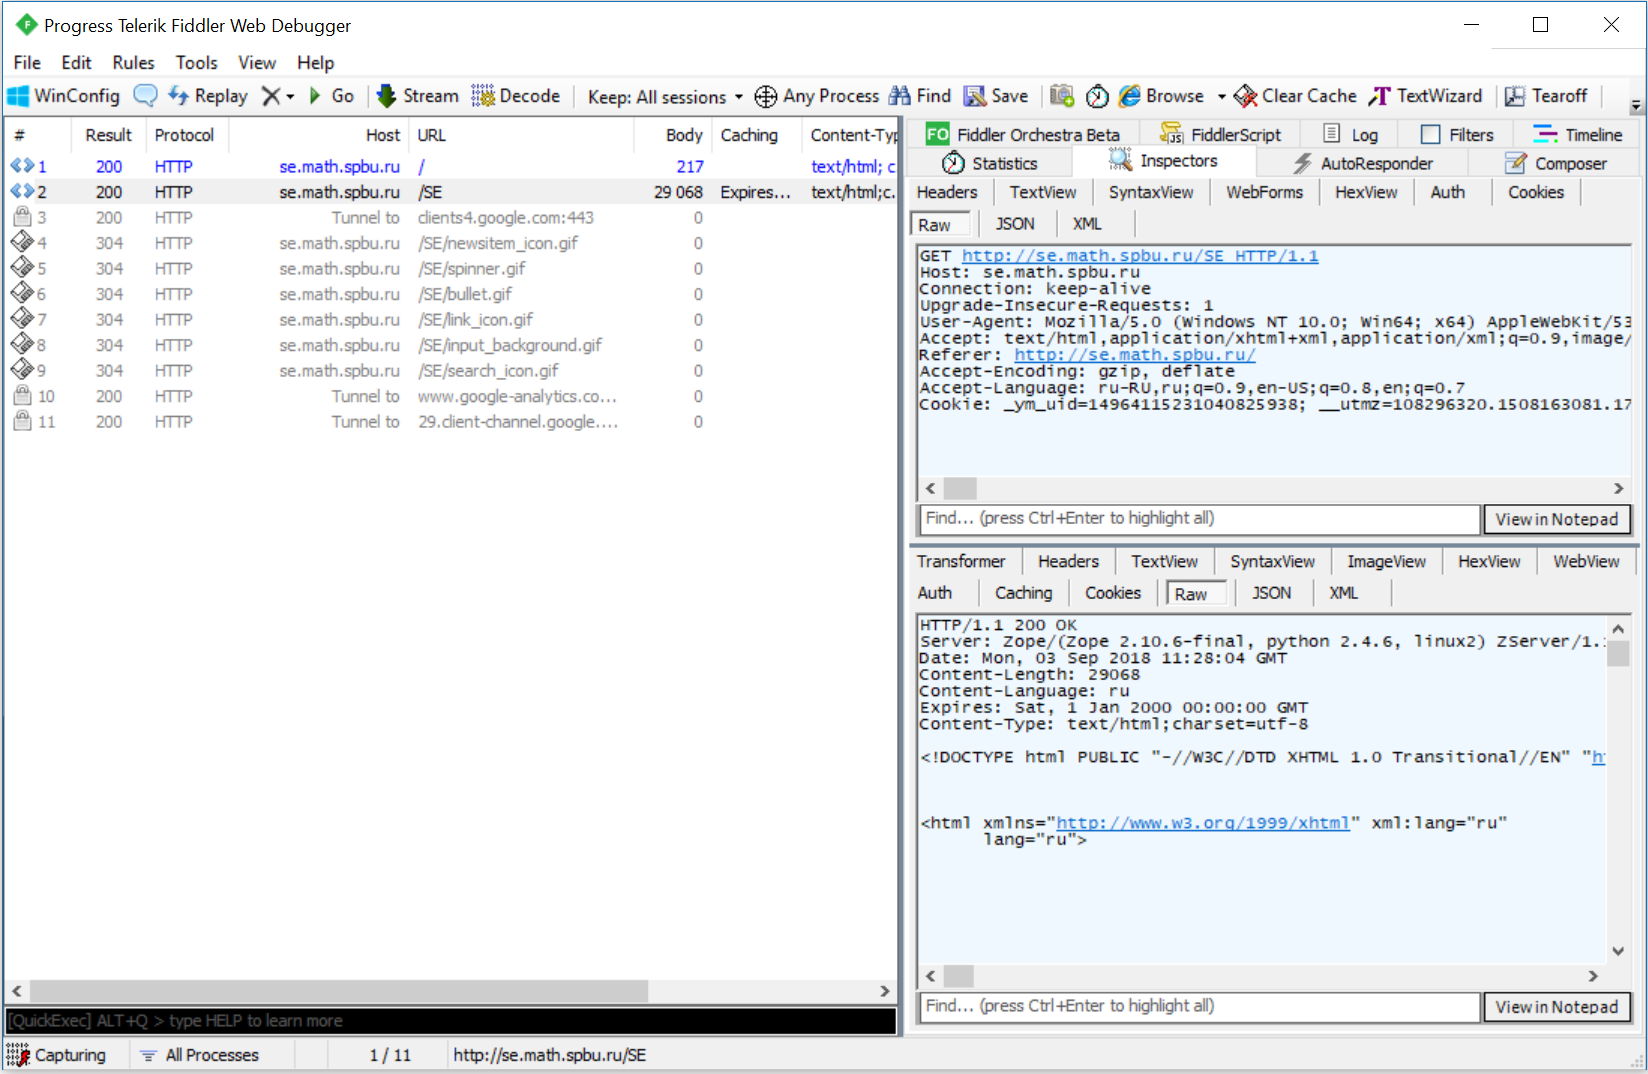
\includegraphics[width=0.9\textwidth]{fiddler.png}
\end{center}

Слева показывается список всех пакетов, отправленных в системе, с используемым протоколом (HTTP/HTTPS), кодом ответа, адресом, URL, размером и т.п. Пакеты можно фильтровать, можно включать/выключать захват пакетов (чтобы обилие сетевого трафика не испортило вам всю отладку). Кликнув на пакет, можно посмотреть на него поближе в окнах справа. Сверху показывается запрос, снизу ответ (если он уже получен). Можно выбирать разные представления, например, Raw --- это просто сырой текстовый вид, можно ещё древовидное JSON- или XML-представление, можно попросить отрендерить HTML-ку как будто в браузере, дешифровать HTTPS-пакет. 

Последнее возможно благодаря тому, что Fiddler умеет подменять сертификат, которым подписывается HTTPS-соединение, устраивая тем самым настоящую Man-In-The-Middle-атаку, разумеется, с ведома и согласия пользователя. Для этого ему надо подсунуть свой сертификат в хранилище доверенных сертификатов ОС, для чего, естественно, требуются администраторские права. Про то, что такое вообще сертификаты, буквально чуть позже в этой же лекции.

\section{Сетевая безопасность}

Теперь -- очень краткая ликвидация безграмотности в области сетевой безопасности. Вообще, эта тема заслуживает отдельного курса, но кое-какие вещи, типа тех же сертификатов, необходимы любому программисту в повседневной работе, так что обойти их обсуждение хотя бы кратко не получится. В современном мире почти все сервисы требуют аутентификации, авторизации и обеспечения безопасности. Причём, обратите внимание, что аутентификацию и авторизацию часто путают, это разные вещи:

\begin{itemize}
    \item \textit{аутентификация} --- это установление личности (точнее, идентичности) участника взаимодействия; личность нам не важна, нам важно знать, что это тот пользователь, о котором мы думаем, или хотя бы пользователь из той группы пользователей с одинаковыми правами, за которого себя выдаёт; аутентификация часто взаимна --- сервер не доверяет клиенту, но и клиент не может быть уверен в том, что сервер не подделан злоумышленником;
    \item \textit{авторизация} --- это установление прав на выполнение операции, когда аутентификация уже выполнена. Вы можете быть вполне легитимным пользователем gmail, но это не значит, что вы имеете право просматривать мою почту; или вы можете иметь доступ только на чтение к какому-то документу.
\end{itemize}

\textit{Шифрование} --- это обеспечение конфиденциальности передаваемой информации. Но для информационной безопасности важна не только конфиденциальность, но и:

\begin{itemize}
    \item \textit{целостность} --- что злоумышлениик ничего не поменял в сообщении; даже не имея возможности его прочитать, он может нанести ущерб, внеся изменения, если они не будут замечены получателем;
    \item \textit{актуальность} --- что злоумышленник не проиграл просто старое сообщение; ведь не надо ни дешифровать, ни изменять как-то ваше сообщение об оплате мобильной связи, чтобы лишить вас всех денег, если протокол оплаты не обеспечивает свойство актуальности.
\end{itemize} 

\subsection{Шифрование}

Классическая схема шифрования предполагает передачу конфиденциальных данных по каналу, который может прослушивать злоумышленник (так наызваемая схема с пассивным злоумышленником) или злоумышленник может модифицировать сообщения в канале (схема с активным злоумышленником):

\begin{center}
    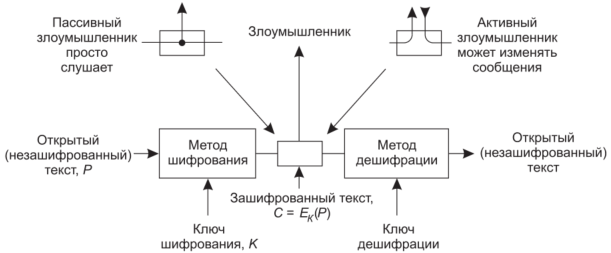
\includegraphics[width=0.8\textwidth]{cryptography.png}
    \attribution{Э. Таненбаум}
\end{center}

Незашифрованынй текст называется в англоязычной литературе Plaintext и поэтому обозначается P. Зашифрованный текст называется Ciphertext и обозначается C. Алгоритм шифрования (Encryption, E) использует параметр K (Key) --- ключ шифрования, по которому преобразует открытый текст в зашифрованный: $C = E_K(P)$. Алгоритм дешифрования (Decryption, D) использует ключ дешифрации (тот же, или отличающийся от K), чтобы построить обратно открытый текст по его зашифрованному варианту.

\noindent\begin{minipage}{\textwidth}
    \begin{minipage}[c][4cm][c]{\dimexpr0.7\textwidth-0.7\Colsep\relax}
        В криптографии традиционно считается, что сам алгоритм шифрования известен, неизвестен только ключ. Связано это с тем, что хороший алгоритм шифрования разработать сложно (это занимает годы) и если его взломают, придётся менять и сам алгоритм, и его программные и аппаратные реализации. Это сложно и дорого. Если взломают ключ, достаточно выбрать другой. Более того, современные алгоритмы заранее меняют ключи раз в несколько секунд, чтобы осложнить злоумышленнику криптоанализ.
    \end{minipage}\hfill
    \begin{minipage}[c][4cm][c]{\dimexpr0.3\textwidth-0.3\Colsep\relax}
        
\includegraphics[width=0.7\textwidth]{youAreBeingWatched.png}
    \end{minipage}%
\end{minipage}

Ещё стоит помнить, что алгоритмы шифрования --- это суровая алгебра, теория чисел и теория вероятностей. Если вы думаете, что криптосхема <<кручу-верчу, запутать хочу>> или последовательное применение двадцати разных алгоритмов шифрования повысит криптостойкость вашего метода шифрации, вас могут ждать неприятные сюрпризы (вплоть до того, что криптостойкость внезапно понизится). Повысить криптостойкость можно увеличением размера ключа, но во многих странах существуют законодательные ограничения на длину ключа в гражданских шифрах. Связано это не с тем, что тоталитарный режим хочет следить за всеми своими гражданами (хотя хочет, конечно), а с тем, что при крайней необходимости (например, постановлении суда) и затратой больших вычислительных ресурсов (например, суперкомпьютера ВМК МГУ) сообщение всё-таки можно было бы расшифровать. Военные шифры имеют такую длину ключа, что дешифровка сообщений по крайней мере грубой силой на всех нынешних и будущих вычислительных ресурсах планеты даже по оптимистичным оценкам займёт время большее, чем нужно Солнцу, чтобы исчерпать запасы водорода и погаснуть.

Подавляющее большинство интернет-трафика шифруется шифрами с симметричным ключом (то есть ключом, одинаковым для шифровки и дешифровки), потому что они работают очень быстро. Обратите внимание, речь идёт не о шифровании секретных донесений шпионов или банковских переводов, а о шифровании вообще всего трафика --- любой веб-страницы, скачиваемых файлов и даже фильмов, которые вы смотрите через стриминговые сервисы (казалось бы, что секретного в фильме, который и так может посмотреть любой желающий, но если посторонние узнают тот факт, что вы его смотрите --- это privacy violation). Поэтому современные процессоры имеют даже аппаратную поддержку симметричных шифров. 

Однако аутентификация и выбор ключа для последующей симметричной передачи выполняются с помощью асимметричных шифров --- шифров, которые используют разные ключи на стороне отправителя и получателя. Асимметричные шифры хороши тем, что могут использовать открытые ключи, которые позволяют отправителю и получателю вообще не обмениваться никакими секретами. 

Как это возможно? Алгоритм шифрования делится на две части, $D$ и $E$ так, что $D(E(P)) = P$ (этим свойством обладает большинство криптосхем). В отличие от симметричного шифрования, протоколы с открытым ключом используют разные ключи от $D$ и $E$ и обладают тем свойством, что ключ от $D$ очень сложно получить, зная только ключ от $E$ (например, для этого надо найти простые сомножители огромного числа или дискретный логарифм по заданному модулю). Ключ от $D$ держится в секрете, ключ от $E$ выкладывается в открытый доступ.

Теперь, положим, Боб хочет послать Алисе сообщение\footnote{Участники взаимодействия по традиции называются Алиса и Боб (А и Б)}. Боб берёт открытый ключ Алисы $E_A$, шифрует им сообщение $P$ и отправляет Алисе. Алиса легко дешифрует сообщение, вычисляя $D_A(E_A(P))$. Злоумышленник не может прочитать сообщение, поскольку не знает $D_A$ и не может его получить. Если Алиса хочет послать сообщение Бобу, она берёт открытый ключ Боба и делает то же, что и Боб. Популярных алгоритмов, построенных по такой схеме, сразу несколько: RSA (основанный на разложении на простые множители), ElGamal (основанный на дискретных логарифмах), эллиптические шифры (основанные вообще на алгебре точек на эллиптических кривых). Все они где-то на самом деле используются.

\subsection{Цифровые подписи}

Шифровать всё сообщение асимметричным шифром слишком трудоёмко, а иногда нам не нужно обеспечить конфиденциальность сообщения, достаточно лишь гарантирвоать, что сообщение было послано тем, кем мы думаем, что они было послано, и не было изменено в процессе передачи. Пример ситуации, когда это нужно --- библиотеки .NET, выкладываемые в NuGet или распространяемые как часть приложений. Было бы не очень здорово, если бы вместо NUnit в NuGet выложили библиотеку, которая собирает данные банковских карточек с любого компьютера, на котором запущена. Для того, чтобы так не было, используются цифровые подписи:

\begin{center}
    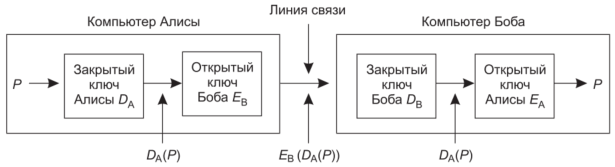
\includegraphics[width=0.8\textwidth]{signature.png}
    \attribution{Э. Таненбаум}
\end{center}

Тут Алиса хочет послать сообщение Бобу так, чтобы Боб мог убедиться, что сообщение действительно послала Алиса, и был бы уверен, что Алиса потом не будет отпираться, что послала сообщение. Алиса сначала шифроует сообщение своим закрытым ключом $D_A$, а затем, как обычно, шифрует то, что получилось, открытым ключом Боба $E_B$. Боб, получив такое сообщение, сначала прменяет свой закрытый ключ, затем открытый ключ Алисы (он его знает, потому что Алиса заранее его опубликовала), получая тем самым исходное сообщение. Он точно знает, что автором была Алиса, потому что если бы автором был кто-то ещё, он бы не знал ключа $D_A$ и при применении $E_A$ получилась бы каша. 

Ну а теперь, собственно, как не шифровать всё сообщение. Давайте сначала по нешифрованному сообщению посчитаем дайджест (Message Digest) --- хорошую хеш-функцию от сообщения, которая обладает таким свойством, что вычисляется по сообщению однозначно, но даже малое изменение сообщения (буквально в одном бите) до неузнаваемости меняет хеш-значение. При этом хеш-функция должна считаться быстро, и по данному хеш-значению должно быть невозможно получить исходное сообщение никак кроме как перебором (что с учётом того, что хеш-функция неизбежно теряет информацию, довольно безнадёжно, перебор даст лишь пару миллионов подходящих сообщений, которые даже похожи на правду). 

Дальше берём посчитанное хеш-значение и подписываем его описанным выше способом только его. Хеш-значение обычно небольшое (например, 20 байт), так что это можно сделать быстро. Адресату шлётся сообщение открытым текстом (например, библиотека .NET) и подписанный хеш (та самая цифровая подпись). Адресат по открытому сообщению сам считает хеш и применяет открытый клю автора к подписанному хешу, сличая то, что получилось. Если хеши одинаковые, то либо сообщение правда было отправлено кем надо и не менялось, либо злоумышленнику удалось подобрать такое сообщение, которое даёт точно то же хеш-значение, что и исходное, и при этом ещё и имеет смысл (что для достаточно хороших хеш-функций статистически маловероятно, настолько, что этим можно пренебречь).

Распространённые криптографические хеш-функции --- это MD5 (старая и уязвимая хеш-функция, коллизии подбираются атакой дней рождения за вполне конечное время), семейство функций SHA (SHA-1, SHA-2, SHA-3). SHA-1 тоже научились ломать, хоть это вычислительно гораздо сложнее, чем MD5, так что для практических цифровых подписей используются более криптостойкие SHA-2 и SHA-3 (SHA-3 относительно новая и не успела стать популярной).

\subsection{Сертификаты}

Окей, теперь мы зная открытый ключ нашего собеседника без проблем проверим, что он тот, за кого он себя выдаёт, но как мы узнаем, что у нас на самом деле правильный открытый ключ нашего собеседника? Понятно, что мы могли бы получить его на флешке, но если бы для того, чтобы ходить во вконтактик, всем пришлось бы ехать за ключом на Невский, никто бы вконтактиком не пользовался. Мы могли бы скачать открытый ключ со страницы нашего собеседника (например, того же vk.com), но злоумышленник довольно без проблем (до сих пор, несмотря на внедрение DNSSec!) может перехватить ваш запрос к странице и отправить вас на свою страницу, которая будет выглядеть точно так же, как vk.com, но содержать открытый ключ злоумышленника. А дальше --- атака Man In The Middle:

\begin{center}
    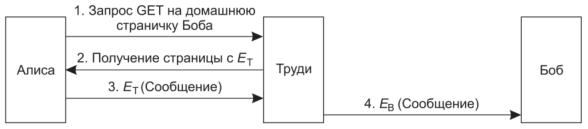
\includegraphics[width=0.8\textwidth]{manInTheMiddle.png}
    \attribution{Э. Таненбаум}
\end{center}

Чтобы такой беды не было, давайте, мм, подписывать открытые ключи. Боб, публикуя свой открытый ключ, получает у кого-то, кому доверяет и Алиса, и Боб, сообщение, что это правда открытый ключ Боба, подписанное этим кем-то, кому все доверяют. Теперь Алиса, получив открытый ключ Боба, может проверить подпись в этом сообщении и убедиться, что это правда ключ Боба. Но что будет, если Труди (от английского inTruder) взломает страницу того, кому все доверяют, и подсунет свой ключ вместо его ключа, заставив тем самым Боба подписать своё ключ фальшивой подписью, которую Труди без проблем сможет подделать во время атаки Man In The Middle? Хм, давайте подпишем и этот ключ, и тот ключ, которым мы подписали этот ключ, и т.д. по цепочки, до Ключа, Которому Точно Все Доверяют. Такой ключ (точнее, несколько десятков их) могут быть вшиты в поставку операционной системы, браузера и т.п., так что при получении сообшщения Алиса может проверить подписи по цепочке до ключа, который она получила от, например, Microsoft, и знает, что у зоумышленника вряд ли хватит денег, чтобы убедить Microsoft подсунуть фальшивый ключ.

Именно так работают \textit{сертификаты}. Сертификат --- это то самое сообщение, подтверждающее идентичность ключа (что-то вида <<предъявитель сего действительно является Иваном Ивановым, владельцем домена example.com>>), подписанное Certificate Authority (CA). Сертификаты имеют фиксированный формат, определяемый стандартом X.509, довольно ужасным, но по сути сводящемся к набору пар <<ключ-значение>>, хранящих информацию о владельце сертификата. Сертификаты бывают разные, от самых простых, что предъявитель сего владеет таким-то доменом, даже без указания имени хозяина, до сертификатов, выдаваемых интернет-магазинам сертификационными центрами, которые подтверждают, что владелец сертификата действительно может заниматься интернет-торговлей, не обманет и достаточно финансово устойчив, чтобы не обанкротиться, пока доставляет вашу покупку.  Понятно, что такие сертификаты стоят денег, и иногда немалых (и выдаются только на время, кстати).

CA верхнего уровня подписывают сертификаты CA уровнем ниже, чтобы те могли подписывать уже сертификаты конечных пользователей. Таким образом, получается цепочка сертификатов от конкретного пользователя до корневого CA, сертификаты которого общеизвестны и им все доверяют. При передаче сообщения передают всю цепочку сертификатов сразу, чтобы для проверки подписей вообще не требовалось выполнять сетевые запросы, благо сертификаты очень небольшие. Получатель может проследить, что все сертификаты в цепочке подписаны друг другом и цепочка заканчивается на сертификате, которому получатель точно доверяет, потому что, например, получил его десять лет назад вместе с новым компьютером. Такие доверенные сертификаты называются корневыми (root certificates) и хранятся в специальном хранилище в ОС любого компьютера.

Поскольку настоящие сертификаты как минимум требуют что-то подтвердить, а как максимум стоят как недорогая иномарка, для отладки сетевых приложений используют \textit{самоподписанные} сертификаты. Это сертификат, который разработчик может сгенерировать сам, ему, понятное дело, никто не доверяет, потому что невозможно отследить его цепочку доверия до корневого сертификата, но разработчик может сам добавить такой сертификат в список доверенных. Тогда все приложения, пользующиеся системными сервисами проверки сертификатов, будут вынуждены ему доверять. Именно так работает Fiddler, когда дешифрует HTTPS-трафик, кстати. Visual Studio, кстати, умеет генерировать самоподписанные сертификаты: \url{https://docs.microsoft.com/en-us/windows/msix/package/create-certificate-package-signing}, но чаще это делают через инструменты библиотеки OpenSSL. 

А вот бесплатное CA, выдающее сертификаты, доказывающие владение доменом: \url{https://letsencrypt.org/}. Ему более-менее все современные браузеры доверяют, так что там можно получить вполне доверенный сертификат, которым можно защищать HTTPS-соединение. Код им подписывать не получится, но по крайней мере, шифровать соединение с сайтом вполне можно (а это необходимо для любого нормального протокола аутентификации). Так что в современном мире неиспользование HTTPS по причине дорговизны сертификата больше не является валидным.

\subsection{HTTPS}

Собственно, сертификаты используются очень много где, но в контексте сетевых приложений они наиболее вахны для установки HTTPS-соединения. HTTPS --- это обычный протокол HTTP, использующий Secure Sockets Layer, или SSL, в качестве протокола уровня представления. Установление соединения по HTTPS включает в себя аутентификацию сервера на клиенте как раз через цепочку сертификатов. Клиент не должен доказывать свою идентичность серверу (об этом потом позаботится аутентификация, уже когда соединение будет установлено), но если сервер не сможет убедить клиента, что он правда тот, на который клиент пытается зайти (в смысле доменного имени), соединение даже установлено не будет.

Вот так примерно устроено установление соединения по HTTPS:

\begin{center}
    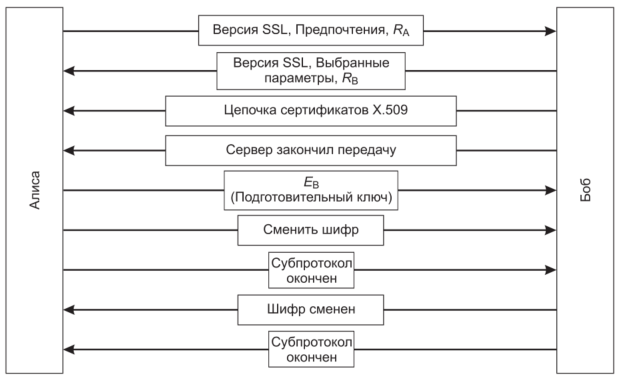
\includegraphics[width=0.8\textwidth]{ssl.png}
    \attribution{Э. Таненбаум}
\end{center}

Сначала Алиса и Боб договариваются о версии SSL и обмениваются одноразовыми ключами (\textit{nonce}, Number used once, просто случайные числа для предотвращения атаки повтором), затем Боб отправляет свою цепочку сертификатов, чтобы доказать, что он правда Боб, затем Алиса шифрует открытым ключом Боба подготовительный ключ для симметричного шифрования (который тоже выбирает случайно, используя nonce-ы), Боб, зная свой закрытый ключ и оба nonce-а, расшифровывает симметричный ключ, подтверждает получение Алисе и переходит на симметричный шифр с этим ключом. Ненадолго, впрочем, HTTPS предполагает частую смену симметричного ключа во избежание статистических атак.

\subsection{OAuth 2}

Последнее, с чем остальнос разобраться --- это с авторизацией. Хорошо, Алиса и Боб смогли подтвердить идентичность друг друга, но Алиса хочет зайти на файловое хранилище и скачать оттуда файл, Боб должен проверить, что она имеет на это право. Боб мог бы сам владеть и файловым хранилищем, и держать у себя таблицу, в которой написано, что Алиса имеет право делать, а что нет, и это бы даже хорошо работало, если бы Алиса только для этого и пользовалась интернетом. Но подумаем об обычном пользователе, который зареган на тысяче ресурсов. Если к каждому надо придумывать свой логин и пароль, можно сойти с ума. Если каждый ресурс знает логин и пароль пользователя, то если взломают хоть один, взломают и все остальные.

Поэтому появился протокол OAuth (тут речь пойдёт про OAuth 2, используемый ныне). Этот протокол позволяет разрешить пользование ресурсом, не раскрывая хозяину ресурса логин и пароль пользователя. Например, можно войти на сторонний ресурс по аккаунту в Google или аккаунту в VK, не сообщая при этом ресурсу никакой ценной информации о себе, не говоря уж о логине и пароле. Так можно помнить только пароль от Google и ходить на все остальные сайты, умеющие в OAuth, по нему. Светлая цель разработки такого протокола была вообще в том, чтобы был некий глобальный сервис аутентификации, которому все доверяют, и который бы позволял проверить идентичность пользователя и дать доступ ко всем остальным сайтам интернетов, но, во-первых, с <<которому все доверяют>> возникли проблемы, во-вторых, когда это человечество о чём-то хорошем договорилось.

Работает протокол примерно как на картинке из стандарта (RFC 6749):

\begin{center}
    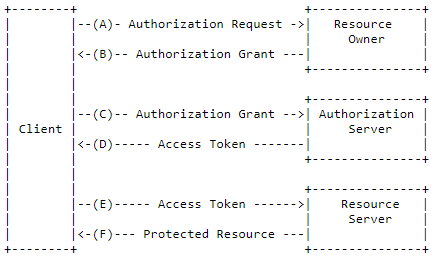
\includegraphics[width=0.6\textwidth]{oauth.png}
    \attribution{RFC 6749}
\end{center}

Client --- это приложение, которое хочет работать с каким-то ресурсом (например, браузерный клиент гуглодиска). Resource Owner --- это пользователь (человек), который может разрешить или не разрешить клиенту доступ к ресурсу. Authorization Server --- это то место, где разрешение на доступ к ресурсу можно обменять на Access Token, если Resource Owner реально имеет право на доступ к ресурсу. Дальше мы можем с этим Access Token-ом пойти на ресурсный сервер и предъявить уже Access Token, чтобы пользоваться ресурсом, не авторизуясь на нём ещё раз. Аутентификация и авторизация проводится только один раз, на Authorization Server-е, выдаваемый им токен устроен так, что Resource Server может легко проверить его валидность и то, что клиент действительно имеет право выполнять запрашиваемую операцию (очередное применение криптографических хешей, кстати).

Чаще всего протокол OAuth 2 используется в режиме Authorization Code, когда клиент не запрашивает у владельца ресурса авторизацию напрямую, а перенаправляет его на Authorization Server, где владелец аутентифицируется и авторизуется. При этом логин/пароль пользователя видит только Authorization Server, даже клиент не имеет к ним доступа. Authorization Server затем отвечает клиенту, отправляя ему Access Token (для чего используется некая магия с URL-ами). При этом Access Token имеет свойство протухать через некоторе небольшое время (чтобы если злоумышленник перехватит Access Token, он с меньшей вероятностью мог воспользоваться ресурсом), поэтому клиенту также обычно выдаётся Refresh Token --- токен, который можно обменять на новый Access Token, когда старый протухнет. Refresh Token живёт подольше (обычно от нескольких дней до пары месяцев) и его можно продлять, так что если пользователь часто пользуется ресурсом (например, ходит во вконтакт каждый день), ему вообще не надо авторизовываться. Refresh Token передаётся по сети довольно редко, так что несмотря на то, что он важнее, вероятность, что его перехватят, меньше. Напомним, что всё происходит по HTTPS, так что чтобы получить хоть один токен, сначала надо взломать относительно неломаемый протокол. А если его всё-таки взломают, Refresh Token часто можно вручную отозвать.

Так устроена большая часть существующих механизмов авторизации для веб-сайтов и веб-сервисов, поэтому с OAuth неплохо бы разобраться и хотя бы раз попробовать.

\end{document}
